\documentclass[10pt,twocolumn,fleqn]{IEEEtran}

%% set page size to US letter
\special{papersize=8.5in,11in}
\setlength{\pdfpageheight}{\paperheight}
\setlength{\pdfpagewidth}{\paperwidth}

\DeclareMathAlphabet{\mathtsl}{OT1}{ptm}{m}{sl}
\RequirePackage{amssymb}
\usepackage{hyperref}
\usepackage{xspace}
\usepackage{algorithm}
\usepackage[noend]{algpseudocode}
\usepackage{amsbsy}
\usepackage{amsthm}
\usepackage{graphicx}
\usepackage{helvet}
\usepackage{enumerate}
\usepackage{amsmath}
\usepackage{amstext}
\usepackage{amsfonts}
\usepackage{graphicx}
\usepackage{multirow}
\usepackage{subfig}
\usepackage{comment}
\usepackage{cases}
\usepackage{xcolor}
\usepackage{epstopdf}
\usepackage[normalem]{ulem}
\usepackage{diagbox}
% \usepackage{titlesec}
% \titlespacing*{\section}{0pt}{1.1\baselineskip}{\baselineskip}

% \newcommand{\B}{{\mathbb{B}}}
\newcommand{\Z}{{\mathbb{Z}}}
\newcommand{\R}{{\mathbb{R}}}
\newcommand{\Q}{{\mathbb{Q}}}
\newcommand{\N}{{\mathbb{N}}}
\newcommand{\C}{{\mathbb{C}}}
\newcommand{\Zn}{{\mathbb{Z}}_{n}}
\newcommand{\Zp}{{\mathbb{Z}}_{p}}
\newcommand{\F}{{\mathbb{F}}}
\newcommand{\FF}{{\mathcal{F}}}
\newcommand{\Fbar}{{\overline{\mathbb{F}}}}
\newcommand{\Fq}{{\mathbb{F}}_{q}}
\newcommand{\Fqbar}{{\overline{{\mathbb{F}}_q}}}
\newcommand{\Fkk}{{\mathbb{F}}_{2^k}}
\newcommand{\Zkk}{{\mathbb{Z}}_{2^k}}
\newcommand{\Fkkx}[1][x]{\ensuremath{\mathbb{F}}_{2^k}[#1]\xspace}
\newcommand{\Grobner}{Gr\"{o}bner\xspace}
\newcommand{\bi}{\begin{itemize}}
\newcommand{\ei}{\end{itemize}}

\newcommand{\idealj}{{J = \langle f_1, \dots, f_s\rangle}}
\newcommand{\idealg}{{J = \langle g_1, \dots, g_t\rangle}}
\newcommand{\vfqj}{{V_{\Fq}(J)}}
\newcommand{\vfkkj}{{V_{\Fkk}(J)}}

%%% Added by Utkarsh %%%
\newcommand{\Va}{{V_A}}
\newcommand{\Vb}{{V_B}}
\newcommand{\Vc}{{V_C}}
\newcommand{\Vbc}{{V_{B,C}}}
\newcommand{\Vabc}{{V_{A,B,C}}}
\newcommand{\Vac}{{V_{A,C}}}
\newcommand{\w}{\wedge}

%%%%%%%%%%%%%%%%%%%%%%%%

\newcommand{\blu}{\color{blue}}
% \newcommand{\Grobner}{Gr\"{o}bner\xspace}
\newcommand{\fqring}{\Fq[x_1,\dots,x_n]}


% New command for the line spacing.
\newcommand{\ls}[1]
    {\dimen0=\fontdimen6\the\font
     \lineskip=#1\dimen0
     \advance\lineskip.5\fontdimen5\the\font
     \advance\lineskip-\dimen0
     \lineskiplimit=.9\lineskip
     \baselineskip=\lineskip
     \advance\baselineskip\dimen0
     \normallineskip\lineskip
     \normallineskiplimit\lineskiplimit
     \normalbaselineskip\baselineskip
     \ignorespaces
    }
% New command for the table bnotes.
\def\tabnote#1{{\small{#1}}}

\newcommand{\beq}{\begin{equation}}
\newcommand{\eeq}{\end{equation}}
\newcommand{\beqarr}{\begin{eqnarray}}
\newcommand{\eeqarr}{\end{eqnarray}}
\newcommand{\ov}{\bar}
\newcommand{\xor}{\bigoplus}
\newcommand{\Fm}{{\mathbb{F}}}
\newcommand{\myfontsize}{\fontsize{7}{9}\selectfont}
\newcommand{\Ftwo}{{\mathbb{F}}_{2}}
\newcommand{\G}{{\mathcal{G}}}
\newcommand{\alert}[1]{\textcolor{red}{#1}}
\newcommand{\B}{{\mathbb{B}}}
\newcommand{\Z}{{\mathbb{Z}}}
\newcommand{\R}{{\mathbb{R}}}
\newcommand{\Q}{{\mathbb{Q}}}
\newcommand{\N}{{\mathbb{N}}}
\newcommand{\C}{{\mathbb{C}}}
\newcommand{\Zn}{{\mathbb{Z}}_{n}}
\newcommand{\Zp}{{\mathbb{Z}}_{p}}
\newcommand{\F}{{\mathbb{F}}}
\newcommand{\FF}{{\mathcal{F}}}
\newcommand{\Fbar}{{\overline{\mathbb{F}}}}
\newcommand{\Fq}{{\mathbb{F}}_{q}}
\newcommand{\Fqbar}{{\overline{{\mathbb{F}}_q}}}
\newcommand{\Fkk}{{\mathbb{F}}_{2^k}}
\newcommand{\Zkk}{{\mathbb{Z}}_{2^k}}
\newcommand{\Fkkx}[1][x]{\ensuremath{\mathbb{F}}_{2^k}[#1]\xspace}
\newcommand{\Grobner}{Gr\"{o}bner\xspace}
\newcommand{\bi}{\begin{itemize}}
\newcommand{\ei}{\end{itemize}}
\newcommand{\idealj}{{J = \langle f_1, \dots, f_s\rangle}}
\newcommand{\idealf}{{F = \{f_1, \dots, f_s\}}}
\newcommand{\idealg}{{J = \langle g_1, \dots, g_t\rangle}}
\newcommand{\vfqj}{{V_{\Fq}(J)}}
\newcommand{\vfkkj}{{V_{\Fkk}(J)}}
\newcommand{\vfqjo}{{V_{\Fq}(J_0)}}
\newcommand{\vfbqj}{{V_{\overline{\Fq}}(J)}}
\newcommand{\vfbqjo}{{V_{\overline{\Fq}}(J_0)}}
\newcommand{\vfbqjjo}{{V_{\overline{\Fq}}(J+J_0)}}
\newcommand{\acf}{\bar{F}_q}
\newcommand{\Vacf}{V_{\bar{F}_q}}
\newcommand{\al}{\alpha}
\newcommand{\w}{\wedge}
\newcommand{\fqring}{\Fq[x_1,\dots,x_n]}
\newcommand{\spec}{{\it Spec}\xspace\ \xspace}

\newcommand{\debug}[1]{\textcolor{gray}{[ #1 ]}}
\newcommand{\blu}{\color{blue}}
\newcommand{\red}{\color{red}}

\theoremstyle{definition}

%the following is for space before and after align or other equation environment.
\newtheorem{Algorithm}{Algorithm}[section]
\newtheorem{Definition}{Definition}[section]
\newtheorem{Example}{Example}[section]
\newtheorem{Proposition}{Proposition}[section]
\newtheorem{Lemma}{Lemma}[section]
\newtheorem{Theorem}{Theorem}[section]
\newtheorem{Proof}{Proof}[section]
\newtheorem{Corollary}{Corollary}[section]
\newtheorem{Conjecture}{Conjecture}[section]
\newtheorem{Problem}{Problem}[section]
\newtheorem{Notation}{Notation}[section]
\newtheorem{Setup}{Problem Setup}[section]

%%set spacing between table columns
\setlength{\tabcolsep}{3pt}
\setlength\intextsep{0pt}

\begin{document}
\setlength{\abovedisplayskip}{0pt}
\setlength{\belowdisplayskip}{0pt}
\setlength{\abovedisplayshortskip}{0pt}
\setlength{\belowdisplayshortskip}{0pt}
\title{\Large\textsc{{R}esolving {U}nknown {C}omponents {I}n {A}rithmetic {C}ircuits {U}sing {C}omputer {A}lgebra {M}ethods}}

\author{Vikas Rao$^1$, Utkarsh Gupta$^1$, Irina Ilioaea$^2$, Priyank Kalla$^1$, and Florian Enescu$^2$\\
$^1$Electrical \& Computer Engineering, University of Utah\\
$^2$Mathematics \& Statistics, Georgia State University \vspace{-0.2in}
}

% \institute{}
\maketitle
\thispagestyle{empty}
%%%%%%%%%%%%%%%%%%%% Include your files here %%%%%%%%%%%%%%%%%%%%%
\begin{abstract}

Resolving an unknown component is a fundamental problem encountered in
post-verification debugging and automatic correction of digital
circuits. Contemporary techniques rely on iterative/incremental
application of SAT solving and Craig interpolation to realize the
functionality of (or resolve) the unknown components. While these
techniques have achieved some success for control-dominated
applications (random logic circuits), they are infeasible in resolving
the unknown components in arithmetic circuits. This paper describes an
algebraic approach to resolve the functionality of an unknown
component in a finite field arithmetic circuit so that the circuit
implementation matches a given specification. Starting from an
equivalence checking setup modeled as a polynomial ideal
membership test in commutative algebra, we formulate the problem of
resolving the unknown component as a quantification procedure. Using
the \Grobner basis algorithm, we derive an approach to identify the
function implemented by the unknown component. We go on to pose the
problem as a synthesis challenge and explore the space of polynomial
functions for the unknown component by analyzing quotients of
ideals. As \Grobner basis algorithms exhibit high computational
complexity, we exploit the circuit topology to improve our
algorithms. We can resolve the unknown components not just for
bit-level circuit implementations, but also in cases where the
abstraction hierarchy is given at the level of (bit-vector)
words. Experiments performed over various finite field arithmetic
circuits demonstrate the efficacy and superiority of our approach as
compared to conventional techniques.

  % Resolving an unknown component is a fundamental problem encountered
  % in logic synthesis for engineering change orders, post-verification
  % debugging and automatic correction of digital circuits. Contemporary
  % techniques rely on the iterative/incremental application of SAT solving
  % and Craig interpolation to realize the functionality of (or resolve)
  % the unknown components. While these techniques have achieved some
  % success for control-dominated applications (random logic circuits),
  % they are infeasible in resolving the unknown components in
  % arithmetic circuits. This paper describes an algebraic approach to
  % resolve the functionality of an unknown component in an arithmetic
  % circuit so that the circuit implementation matches a given
  % specification. Our approach is formulated as a polynomial ideal
  % membership test. We go on to pose the problem as a synthesis
  % challenge and explore the solution space of the unknown component
  % using concepts from the quotient of ideals. We propose a \Grobner basis 
  % based algorithm for a systematic, goal driven search for
  % implementable solutions. The paper presents results on some
  % experiments performed over various finite field arithmetic circuits
  % to compare the efficiency of our approach against recent methods.   


% Automatic bug correction is a tedious and resource intensive process. 
%% Automatic correction of unknown components in a given circuit is a
%% resource intensive process. Recent developments in realizing the
%% functionality implemented by these unknown gates rely on incremental
%% SAT solving. Despite using state-of-the-art SAT solvers, these
%% approaches fail to verify multipliers beyond 12-bits and hence are
%% infeasible in a practical setting. The current formal datapath
%% verification methods which utilize symbolic computer algebra concepts,
%% rely heavily on textbook structure of the circuits to realize an
%% unknown component, and hence are not scalable. These approaches model
%% circuit as a set of polynomials over integer rings, and use function
%% extraction, simulation, and term rewriting using coefficient
%% computation to arrive at a solution. The approach is not complete in
%% the sense that the procedure cannot be extended to random logic
%% circuits and finite field circuits due to ambiguities in coefficient
%% computation. The approach also fails to verify circuits when redundant
%% gates are introduced in the design. To overcome all these limitations,
%% this paper describes a formal approach using finite field theory to
%% automatically realize the function implemented by an unknown
%% component, and verify the same. The paper introduces theory on
%% resolving a single unknown component using ideal membership testing
%% and \Grobner basis based reduction. We go onto pose the problem as a
%% synthesis challenge and extend the solution space of the unknown
%% component using concepts from quotient of ideals. Since the solution
%% space is not unique, we will also discuss a systematic, goal driven
%% search for simple implementable solutions. The paper presents results
%% on some preliminary experiments performed over various arithmetic
%% circuits to compare efficiency of our approach against recent methods.  
\end{abstract}

%\section{Introduction}
Verifying functional correctness of gate-level arithmetic circuits is still a significant challenge owing to ever increasing design size and functional complexity. A considerable amount of manual intervention is required to localize a bug and correct it, thus making it a resource intensive process. Traditional automated debugging techniques based on simulation, decision procedures such as Binary Decision Diagrams (BDDs)~\cite{bryant:1} and SAT solvers~\cite{alanmi:2006} demand bit-blasting of the circuit, and are hence considered inefficient models to verify complex datapath designs. Due to the inherent algebraic nature of computations in such designs, symbolic algebra algorithms are considered more appropriate for their verification.

Under symbolic algebra environment, a given specification and its circuit implementation are modeled as a set of polynomials. The verification problem is then formulated as \textit{membership testing}~\cite{gb_book} which can prove/disprove whether the circuit implements the specification. In the case of buggy circuits the verification fails; faulty gate(s) are identified and a correction is computed to rectify the circuit. The paper considers a single gate fault model i.e., exactly one of the gates in the circuit is incorrectly synthesized thereby implementing a wrong function at its output. For example, an AND gate replaced with an XOR gate. Once a particular gate has been identified as buggy, we label this gate as the \textit{unknown component}. We propose an approach to realize a correction function which can be implemented at the output of this \textit{unknown component}, such that the entire circuit implementation conforms to the specification. Identifying the buggy gate in a given circuit implementation is a much harder problem and is in the future scope of our work. This paper puts forth the underlying theory on realizing and exploring the solution space for correction functions, and outlines the future verification challenges.
\vspace{-0.1in}
\subsection{Previous work}

The most recent and relevant approach~\cite{fujita:2015},~\cite{fujita:2012} resolves the unknown component problem using an incremental $SAT$ formulation. The paper models the unknown component in a given circuit($Ckt$) as a LUT by using transformation variables($X$). The solution to these variables implements the desired logic function so that the resulting circuit becomes logically equivalent to a given specification $Spec()$. Let $Ckt(X,In)$ be the formula corresponding to the given circuit with possible transformations, where $In$ is the set of all primary inputs to the circuit. This can be formulated naturally as a two-level QBF with a existential quantifier followed by a universal quantifier as shown below:
\vspace{0.1in}
\begin{align}
\exists \textit{X}.\forall \textit{In. Ckt(X,In) = Spec(In)}:    
\end{align}

The two level QBF is then solved by repeatedly applying the below SAT formulation:
  
\begin{enumerate}
	\item Let Target=($Ckt(X,In)\neq spec(In))$. Let $k$ be the num-ber of test vectors, initialized to zero. Let $TestSet$ be the set of all generated test patterns, initialized to the empty set.
	\item Check if Target is satisfiable.
	\item If SAT, $k=k+1$ and record the solution as $TestSet = TestSet \cup in_k$. The Target is then updated as Target = (Target($X,In))\land(Ckt(X,in_k)=Spec(in_k))$, and go to step 2.
    \item If UNSAT, we have all the required test set patterns $\{in_1$ $\dots in_k\}$. Now, check if: $(Ckt(X,in_1) = Spec(in_1)) \land (Ckt(X,in_2) = Spec(in_2)) \land \dots (Ckt(X,in_k) = Spec$ $(in_k))$ is satisfiable.
    \item If SAT, then any solution $X$ is a correct set of transformation, while an UNSAT result proves that there does not exist a correct set of transformation.
\end{enumerate}

% By experiment, the approach shows that if the circuit is correct under these input patterns($in_k$), it is guaranteed to be correct for all of $2^{In}$ input patterns.
The work in~\cite{maciej:2017} poses the unknown component formulation as a camouflaged circuit model and tries to de-obfuscate several types of camouflaging techniques using incremental SAT solving. The approach used in~\cite{andreas:2005} inserts logic corrector MUXs on the unknown sub-circuits and relies on SAT solvers to realize the functionality. 

Despite using state-of-the-art SAT solvers, all the above approaches fail to verify large and complex finite field arithmetic circuits. The solvers still model the problem as decision procedures and, as demonstrated by our experimental results, are shown to be inefficient in solving verification problems on multiplier circuits beyond 12-bits. 

The technique from Farahmandi et al.~\cite{farimah:2016} deals with automatic debugging and correction using computer algebra concepts. The authors use function extraction~\cite{maciej:2015:1} with a specific term order~\cite{lv} to do equivalence checking, subsequently generating a remainder in case of failure. The approach then finds all possible assignments to variables of the remainder such that it generates a non-zero value. This test set helps arrive at a pruned gate list for bug localization. The procedure then takes every gate in the pruned list, starting from primary inputs, and tries to match the appeared remainders pattern. It does so by computing the difference between the polynomial computed at the output of the suspicious gate against the polynomial computed by a probable set of gate corrections. The coefficient computation~\cite{maciej:2015:2} during pattern matching relies heavily on the half-adder based circuit structure. The paper doesn't discuss the ambiguities in weight calculations when the gate structure differs from the given topology. The approach is not complete in the case when there are redundant gates in the circuit as we found through our experiments. The approach also doesn't talk about finite field arithmetic circuits as the experiments are illustrated with only integer arithmetic circuits.

% and hence The approach also fails to arrive at a conclusive solution when the circuit is tweaked with some redundancy and hence lacks completeness. 

% While theorem provers require extensive manual intervention and expertise. 

% Additional constraint relating floating signals to fanouts in the circuit must be satisfied for the result to be trusted; however the computation to verify this condition can be expensive. For this reason, this method becomes inefficient if the number of logic gates dominates the HA network. Also, the circuit would need to be partitioned into linear and non-linear portions, which is a non-trivial task.

% \subsection{Contribution}
% % by extending it to random logic circuits. 
% The paper discusses a single gate replacement error model as the target design i.e., only one gate in the design incorrectly replaced, for example an AND gate replaced with an XOR/OR gate. We are given a circuit implementation $C$, modeled as a set of polynomials $F=\{f_1,\dots,f_s\}$, with one of these gates $f_i$ marked as unknown component. We then utilize concepts from symbolic computer algebra to realize the function implemented by this unknown component. The reference golden model can either be a specification polynomial $f$ or a different circuit $C_1$ implementing the same function as circuit $C$. For a given specification polynomial $f$, we do polynomial reduction until the unknown component gate and arrive at the function implemented by the component by using \Grobner basis based guided ideal membership testing, and elimination ideal. For the case where the specification is given in terms of a different implementation $C_1$, we use \Grobner basis based reduction on a miter setup to arrive at a solution. %, and apply $\it{Nullstellensatz}$ principles to verify the function implemented by the component%
% This paper seeks to put forth the underlying theory, outline the verification challenges, and present a complete approach to resolve an unknown component in finite field arithmetic circuits. We also discuss some preliminary but encouraging experimental results and draw a comparison to the SAT-based approach.  

% The paper will address both the notions by analyzing the circuit polynomials using concepts from computer algebra\cite{gb_book}\cite{ideals:book} such as \Grobner basis reduction, projection of variety, elimination ideal, ideal membership testing, and weak $\it{Nullstellensatz}$.

%Extra
% Partial synthesis required for logic optimization and Engineering Change Order(ECO). Design is treated as a combinatorial black box, and in order to determine the logic function realized by the design, it is necessary to constraint the circuit topologically. A set of sub-circuits considered as vacant with fixed inputs are treated used for transformation to realize the function implemented by the unknown component.
%\vspace{-0.1in}
\section{Notation and Preliminary Concepts}
\label{sec:prelim}
Let $\Fq$ denote the finite field of $q$ elements where $q=p^k$ is a
prime power, $\Fqbar$ be its algebraic closure, and $R = \fqring$ the
polynomial ring in $n$ variables $x_1,\dots,x_n$, with coefficients
from $\Fq$. A monomial is a power product of the form  $X =
x_1^{e_{1}}\cdot x_2^{e_{2}}\cdots x_n^{e_{n}}$, where  
$e_i \in \Z_{\geq 0}, i\in \{1, \dots,n\}$. A {\it polynomial} $f \in
R$ is written as a finite sum of terms   
$f = c_1 X_1 + c_2 X_2 + \dots + c_t X_t$, where $c_1, \dots, c_t$ are 
coefficients and $X_1, \dots, X_t$ are monomials. Impose a monomial
order $>$ (a term order) on the ring -- i.e. a total order and a
well-order on all the monomials of $R$ s.t. multiplication with
another monomial preserves the order. Then the monomials of all
polynomials $f = c_1 X_1 + c_2 X_2 + \dots + c_t X_t$ 
are ordered w.r.t. to $>$, such that  $X_1 > X_2 > \dots >  X_t$.
Subject to $>$, $lt(f) = c_1 X_1, ~lm(f) = X_1, ~lc(f) = c_1$,
are the {\it leading term}, {\it leading monomial} and {\it   leading
  coefficient} of $f$, respectively. In this work, 
we consider mostly with lexicographic (lex) term orders.

\subsubsection{Ideals, Varieties and Gr\"obner Bases:} 
Given a set of polynomials $F = \{f_1, \dots, f_s\}$ in $R$, the {\it
  ideal} $J \subseteq R$ generated by them is: %\vspace{-0.1in} 
$J = \langle f_1, \dots, f_s \rangle = \{\sum_{i=1}^{s} h_i\cdot f_i:
~h_i \in R\}.$ The polynomials $f_1, \dots, f_s$
form the {\it basis} or the {\it   generators} of $J$.    


Let $\bm{a} = (a_1,\dots,a_n) \in \Fq^n$ be a point in the affine
space, and $f$ a polynomial in $R$. If $f(\bm{a}) = 0$, we say
that $f$ {\it vanishes} on $\bm{a}$. We have to
analyze the {\it set of all common zeros} of the polynomials of $F$
that lie %$\{f_1, f_2,\dots, f_s\}$ 
within the field $\Fq$. This zero set is called the {\it variety}. It
depends not just on the given set of polynomials but rather on the
ideal generated by them. We denote it by $V_{\Fq}(J) =
V_{\Fq}(f_1,\dots,f_s)$, where: 
$$V_{\Fq}(J) = V_{\Fq}(f_1, \dots, f_s) = \{\bm{a} \in \Fq^n: \forall
f \in J, f(\bm{a}) = 0\}.$$

Varieties can be different when restricted to the given field $\Fq$
or considered over its algebraic closure $\Fqbar$. We will generally
drop the subscript when considering varieties over $\Fq$ and
denote $V(J)$ to imply $V_{\Fq}(J)$. The subscripts will be used,
however, to avoid any ambiguities, e.g. when comparing $V_{\Fq}(J)$
against the one over the closure $V_{\Fqbar}(J)$. 

Given two ideals $J_1 = \langle f_1,\dots,f_s\rangle, J_2=\langle
h_1,\dots,h_r\rangle$, the sum $J_1 + J_2 = \langle
f_1,\dots,f_s,h_1\dots,h_r\rangle$, and their product $J_1\cdot J_2 =
\langle f_i\cdot h_j: 1\leq i\leq s, 1\leq j\leq r\rangle$. Ideals and
varieties are dual concepts: $V(J_1 + J_2) = V(J_1) \cap V(J_2)$, and
$V(J_1\cdot J_2) = V(J_1) \cup V(J_2)$. Moreover, if $J_1 \subseteq
J_2$ then $V(J_1)\supseteq V(J_2)$.

%is an ideal, and so is their
%intersection $J_1\cap J_2$. 
%The union of ideals is, in general, not an
%ideal; however, $J_1 + J_2$ is the smallest ideal containing $J_1
%\cup J_2$. 



\underline{\it Gr\"obner Basis:} An ideal may have many different sets
of generators:  $J = \langle f_1,\dots,f_s\rangle = \dots = \langle
g_1,\dots,g_t\rangle$. Given a 
non-zero ideal $J$, a {\it Gr\"obner 
  basis} (GB) for $J$ is a finite set of polynomials $G = \{g_1,\dots,
g_t\}$ satisfying $\langle \{lm(f) ~|~ f \in J\} \rangle = \langle
lm(g_1),\dots,lm(g_t)\rangle$. Then $J = \langle G \rangle$ holds and
so $G=GB(J)$ forms a basis for $J$. A GB $G$ possesses important
properties that allow to solve many polynomial computation and
decision problems. The famous Buchberger's algorithm (see Alg. 1.7.1 
in \cite{gb_book}) takes as input the set of polynomials $F =
\{f_1,\dots,f_s\}$ and computes the GB
$G=\{g_1,\dots,g_t\}$. A GB can be {\it reduced} to eliminate
redundant polynomials from the basis. A reduced GB is a canonical
representation of the ideal. In this work, the set $G$ will denote a
reduced GB, and any reference to computation of an ideal can be 
construed as constructing its GB.  
%Also, when we reason about properties of ideals
%(interpolants), the reader may assume that a $G = GB(J)$ has been

\subsubsection{Varieties over finite fields and the structure of
  Gr\"obner bases:} When the variety of an ideal is finite, then the
ideal is said to be {\it zero-dimensional}. As $V_{\Fq}(J)$ is a
finite set, $J$ is zero-dimensional. 
%% As we operate over finite fields $\Fq$, which
%% are a finite set of points, we are concerned only with
%% zero-dimensional ideals.  
A GB for a zero dimensional ideal exhibits a 
special structure that we exploit in this work. 

For all elements $\alpha \in \Fq, \alpha^q = \alpha$. Therefore, the
polynomial $x^q-x$ vanishes everywhere in $\Fq$, and is called the
vanishing polynomial of the field, sometimes also referred to as the
field polynomial. Denote by $J_0 = \langle
x_1^q-x_1,\dots,x_n^q-x_n\rangle$ the ideal of all vanishing
polynomials in the ring $R$. Then $V_{\Fq}(J_0) = V_{\Fqbar}(J_0) =
\Fq^n$. Therefore, given any ideal $J$, $V_{\Fq}(J) = V_{\Fqbar}(J)
\cap\Fq^n = V_{\Fqbar}(J) \cap V_{\Fqbar}(J_0) = V_{\Fqbar}(J+J_0) =
V_{\Fq}(J+J_0)$. 



\begin{Theorem}[{\it The Weak Nullstellensatz over finite fields (from
      Theorem 3.3 in \cite{gao:gf-gb-ms})}]
\label{thm:weak-ns-ff}
{\it For a finite field $\Fq$ and the ring $R = \Fq[x_1, \dots, x_n]$, let
$J = \langle f_1, \dots, f_s\rangle \subseteq R$, and let $J_0 = \langle
x_1^q-x_1, \dots, x_n^q -  x_n\rangle$ be the ideal of vanishing
polynomials. Then $V_{\Fq}(J) = \emptyset \iff 1 \in J + J_0 \iff G =
reducedGB(J+J_0) = \{1\}$. }
\end{Theorem}

To find whether a set of polynomials $f_1,\dots,f_s$ have no common
zeros in $\Fq$, we can compute the reduced GB $G$ of
$\{f_1,\dots,f_s,x_1^q-x_1,\dots,x_n^q-x_n\}$ and see if $G = \{1\}$. If
$G\neq\{1\}$, then $f_1,\dots,f_s$ do have common zeros in $\Fq$, and
$G$ consists of the finite set of polynomials $\{g_1,\dots,g_t\}$ with the
following properties. 

\begin{Theorem}[{\it Gr\"obner bases in finite fields (application of
      Theorem 2.2.7 from \cite{gb_book} over $\Fq$)}]
\label{thm:gb-finite}
{\it For $G = GB(J+J_0) = \{g_1,\dots,g_t\}$, the following statements
  are equivalent:
\begin{enumerate}
\item The variety $V_{\Fq}(J)$ is finite.
\item For each $i = 1,\dots, n$, there exists some
$j\in\{1,\dots,t\}$ such that $lm(g_j) = x_i^l$ for some $l\in
\mathbb{N}$. 
\item The quotient ring ${\Fq[x_1\dots,x_n]}\over{\langle G\rangle}$ forms a
  finite dimensional vector space.
\end{enumerate}
}
\end{Theorem}

In other words, the ideal $J+J_0$ is zero-dimensional, and for each
variable $x_i$, there exists an element in the GB whose leading term
is a pure power of $x_i$. When that happens, we can also count the
number of solutions. For a GB $G$, let $LM(G)$ denote the set of 
 leading monomials of all elements of $G$: $LM(G) =
 \{lm(g_1),\dots,lm(g_t)\}$.  

\begin{Definition}[{\it Standard Monomials}]
Let $\bm{X^e} = x_1^{e_1}\cdots x_n^{e_n}$ denote a monomial. The set
of standard monomials of $G$ is defined as 
$ SM(G) = \{\bm{X^e} : \bm{X^e} \notin \langle LM(G) \rangle\}.$
\end{Definition}

\begin{Theorem}[{\it Counting the number of solutions (Theorem 3.7 in
      \cite{gao:gf-gb-ms})}] 
\label{thm:count}
{\it
Let $G = GB(J+J_0)$, and $|SM(G)| = m$, then the ideal $J$ vanishes on
$m$ distinct points in $\Fq^n$. In other words, $|V(J)| = |SM(G)|.$
}
\end{Theorem}

%% We demonstrate the application of these results using an example.

%% \begin{Example}
%% Consider the ideal $J_A = \langle ab, bd, bc + c, cd, bd + b + d + 1
%% \rangle \subset \F_2[a,b,c,d]$ and $J_0 = \langle a^2 - a,b^2 - b,c^2
%% - c,d^2 -d \rangle$. Using a lex term order with $a > e > b > c > d$,
%% compute $G = GB(J+J_0) = \{cd, b+d+1 \}

%% \end{Example}
%\include{exm1}

\subsection{Radical ideals and the Strong Nullstellensatz} 
\begin{Definition}
Given an ideal $J\subset R$ and $V(J) \subseteq \Fq^n$, the {\it ideal
of polynomials that vanish on} $V(J)$ is $I(V(J)) = \{ f \in R :
\forall \bm{a} \in V(J), f(\bm{a}) = 0\}$.
\end{Definition}

If $I_1 \subset I_2$ are ideals then $V(I_1) \supset V(I_2)$, and
similarly if $V_1 \subset V_2$ are varieties, then $I(V_1) \supset
I(V_2)$. 

\begin{Definition}
For any ideal $J\subset R$, the {\bf radical} of $J$ is defined
as $\sqrt{J} = \{f \in R: \exists m \in \mathbb{N} s.t. f^m \in J\}.$
\end{Definition}

When $J = \sqrt{J}$, $J$ is called a radical ideal. Over algebraically
closed fields, the {\it Strong Nullstellensatz} establishes the
correspondence between radical ideals and varieties. Over finite
fields, it has a special form. 


\begin{Lemma}
\label{lemma:radical-ff}
(From \cite{gao:qe-gf-gb}) For an arbitrary ideal $J\subset
\Fq[x_1,\dots,x_n]$, and  $J_0 = \langle
x_1^q-x_1,\dots,x_n^q-x_n\rangle$, the ideal $J + J_0$ is radical; 
i.e. $\sqrt{J+J_0} = J+J_0$. 
\end{Lemma}


\begin{Theorem}[{\it The Strong Nullstellensatz over finite fields
   (Theorem 3.2 in \cite{gao:qe-gf-gb})}] \label{thm:strong-ns}  
For any ideal $J \subset \Fq[x_1,\dots,x_n], ~I(V_{\Fq}(J)) = J + J_0$.
\end{Theorem}

%% \begin{proof}
%% $I(V(J)) = I(V_{\Fq}(J))  = I(V_{\Fqbar}(J + J_0) = \sqrt{J+J_0} = J + J_0$.
%% \end{proof}

\subsection{Projection of varieties and elimination ideals in finite
  fields} 

\begin{Definition}
Given an ideal $J = \langle f_1,\dots, f_s \rangle \subset R$ and its
variety $V(J) \subset \Fq^n$,  
the $l$-th projection of $V(J)$ denoted as $Pr_l(V(J))$ is the mapping
\begin{center}
$Pr_l(V(J)):\Fq^n \rightarrow \Fq^{n-l}, ~Pr_l(a_1,\dots,a_n) = (a_{l+1},\dots,a_n) $
\end{center}
for every $\bm{a} = (a_1,\dots,a_n) \in V(J)$.
\end{Definition}
% The projection of variety of $J_A$ from Example \ref{example:ja} on
% the variable set $C$ is $Pr_A(\Vac(J_A))$ and is equal to $(bcd):\{100,110,001\}$.

\begin{Definition}
Given an ideal $J \subset \Fq[x_1,\dots,x_n]$, the $l$-th elimination
ideal $J_l$ is an ideal in $R$ defined as $J_l = J \cap \Fq[x_{l+1},\dots,x_n]$.
\end{Definition}

The next theorem shows how we can obtain the generators of the $l$-th
elimination ideal using Gr\"obner bases.

\begin{Theorem}[{\it Elimination Theorem \cite{ideals:book}}]
Given an ideal $J \subset R$ and its GB $G$ $w.r.t.$ the
lexicographical (lex) order on the variables 
where $x_1 > x_2 > \cdots > x_n$, then for every $0 \leq l \leq n$ we
denote by $G_l$ the GB of $l$-th elimination ideal of $J$ and compute it as:
\begin{center}
$G_l = G \cap \Fq[x_{l+1},\dots,x_n]$
\end{center}
\end{Theorem}
% The elimination ideal corresponding to $J_A$ from Example \ref{example:ja}
% that eliminates the variables from the set $A$ is 
% $\langle cd,b+d+1 \rangle$ and its variety $\{001,100,110\}$.

In a general setting, the projection of a variety is a subset of the
variety of an elimination ideal: $Pr_l(V(J)) \subseteq V(J_l)$. However,
operating over finite fields, when the ideals contain the vanishing
polynomials, then the above set inclusion turns into an equality.


\begin{Lemma}[Lemma 3.4 in \cite{gao:qe-gf-gb}]
\label{lemma:project}
Given an ideal $J \subset R$ that contains the vanishing polynomials of 
the field, then $Pr_l(V(J)) = V(J_l)$, 
i.e. the $l$-th projection of the variety of ideal $J$ is equal to 
the variety of its $l$-th elimination ideal.

\end{Lemma}

%% \begin{Theorem}[Extension Theorem \cite{coxbook}] 
%% Given the ideal $J \in R$ and its first elimination ideal $J_1$,
%% write each generator $f_i (1\leq i\leq s)$ of $J$ in the form,
%% \begin{center}
%% $f_i = h_i(x_2,\dots,x_n)\cdot x_1^{N_i} + \text{monomials with degree of $x_1 < N_i$}$,
%% \end{center}
%% where $N_i \geq 0$ and $h_i \in \Fq[x_2,\dots,x_n]$ is non-zero. Let's say that there is
%% point $(a_2,\dots,a_n)$ in $V(I_1)$. If $(a_2,\dots,a_n) \not \in V(h_1,\dots,h_s)$,
%% then there exists $a_1 \in \Fq$ such that 
%% $(a_1,a_2,\dots,a_n) \in V(J)$.   
%% \end{Theorem}

%% In other words, if the condition $(a_2,\dots,a_n) \not \in V(h_1,\dots,h_s)$ is satisfied,
%% then the point $(a_2,\dots,a_n) \in V(I_1)$ can be extended to a point
%% $(a_1,a_2,\dots,a_n) \in V(J)$.
%% \par For an ideal $J$ that contains the vanishing polynomials, its GB
%% $G = \{g_1,\dots,g_t\}$ has the property that for each variable in $\{x_1,\dots,x_n\}$
%% there must be some polynomial $g_i$ such that $lm(g_i) = x_i^l$ for $l \in \mathbb{N}$.
%% Therefore, every point in $V(G_l)$ can be extended to a point in $V(G)$.  

We will utilize all of the above concepts to derive the results in
this paper. 

%\section{Theory and Procedure}
\label{sec:theory}
In this section we describe the procedure and algorithm used to arrive at a function implmentable for the unknown component and also show how we can explore the solution space. We will apply the algorithm on an example to substantiate our theory. 
\subsection{Reference specification is polynomial f}
Consider a specification polynomial $f$ and its circuit implementation $C$, modeled as polynomials $F = \{f_1,\dots,f_s\}\in \mathbb{F}_q[x_1,\dots, x_n]$. The generator of polynomials is given as $J=\langle F \rangle$, with $J_0=\langle x_l^q-x_l\rangle$ being the set of all vanishing polynomials. Let us consider RTTO (\autoref{def:rtto}) as the variable order for the circuit. We will assume $f_i:1\le i \le s$ to be the unknown component which is of the special form:
\begin{gather} 
\label{fiform}
f_i = x_i + P(X_u)
\end{gather}

where $x_i$ is the leading monomial, and $P$ is the tail representing desired solution in variables$:X_u \subset \{x_1,\dots,x_n\} \text{ s.t. } x_j \in X_u \text{ and } x_j<x_i$ in the order. 

As described in ~\autoref{lem:imt} for a correct implementation, specification $f$ should vanish on the variety of ideal generated by the circuit polynomials i.e., $f$ will be in the ideal generated by the circuit:

\begin{equation}
\label{member}
f \in J + J_0; 
f \in \langle f_1,..,f_s\rangle + \langle x_l^q-x_l\rangle;1\le l \le n
\end{equation}
% $f = h_1f_1 + h_2f_2 +\dots+h_if_i+\dots+h_sf_s+H\langle x_i^q-x_i\rangle$
Using Ideal membership testing, we can rewrite $f$ in terms of its generators as:

$f = h_1f_1 + h_2f_2 + \dots+h_if_i+\dots+h_sf_s +H\langle x_l^q-x_l\rangle$

where $H, h_m:1\le m \le s$ are arbitrary elements from $\Fq$.\\
From~\eqref{fiform}:

% $f = h_1f_1 + h_2f_2 +\dots+h_ix_i+h_iP+\dots+h_sf_s+H\langle x_i^q-x_i\rangle$
{\small$f = h_1f_1 + h_2f_2 +\dots+h_ix_i+h_iP(X_u)+\dots+h_sf_s+H\langle x_l^q-x_l\rangle$}

% Given the RTTO $>$, we know the polynomials from $f_s,\dots,f_{i+1}$ and the leading term of $f_i$. Using algorithm:(\ref{algo:mv_reduce}) to reduce 
% $f - h_1f_1 - h_2f_2 -\dots-h_ix_i = h_iP+\dots+h_sf_s+H\langle x_i^q-x_i\rangle$
$f - h_1f_1 -\dots-h_ix_i = h_iP(X_u)+\dots+h_sf_s+H\langle x_l^q-x_l\rangle$

% $f - h_1f_1 - h_2f_2 -\dots-h_ix_i \in \langle h_i,f_{i+1},\dots,f_s, x_i^q-x_i\rangle$
$f - h_1f_1 -\dots-h_ix_i \in \langle h_i,f_{i+1},\dots,f_s, x_l^q-x_l\rangle$\\
We shall call the intermediate remainder computed on the left hand side as $g$.
\begin{equation}
g \in \langle h_i,f_{i+1},\dots,f_s, x_l^q-x_l\rangle
\end{equation}
Given polynomials $h_i, g, f_{i+1},\dots,f_s$, we compute $P$ such that:

 $g = P*h_i+h_{i+1}f_{i+1}+\dots+h_sf_s+H\langle x_l^q-x_l\rangle$

The computed $P$ is a solution to the function implemented by the unknown gate. This linear combination computation is done using $lift$ (\autoref{lem:imt}) implementation in SINGULAR~\cite{DGPS_410}.

%add this as a lemma
We will also have cases, when $h_i$ ends up being a constant, in which case $lift$ returns $g$ itself as a solution $h_i^{'}$. To arrive at a implementable solution, we divide $h_i^{'}$ by the constant $h_i$(multiply the inverse of $h_i$) and reduce the result by rest of the input polynomials\{$f_{i-1},\dots,f_1$\}. 

\begin{align}
h_i^{'}*h_i^{-1}\xrightarrow[]{f_{i+1}}\xrightarrow[]{f_{i+2}}\dots\xrightarrow[]{f_s}P
\end{align}
Despite being a correct solution, the above approach doesn't guarantee the solution to be in the immediate support variables of $f_i$ due to RTTO$>$. To determine a solution in immediate support variable set $x_j$ of $f_i$, we use an elimination term order (\autoref{def:elim}) for the variables $x_k$ followed by $x_j$. We can then compute a $GB$ using this elimination term order with the intermediate solution $P$ added as tail of $f_i$. This $GB$ will have one and only one polynomial which is of the form $x_k + \mathcal{F}(x_j)$, where $\mathcal{F}$ is the function implemented by the gate, and is the most desired solution. 

Since we found two solutions, it is given that $P$ is not unique. We can explore more such solutions which might satisfy the unknown component functionality. Given $P$ as one of the solutions, under RTTO$>$ we have:

$g = P*h_i+h_{i+1}f_{i+1}+\dots+h_sf_s+H^{'}\langle x_l^q-x_l\rangle;$\\
Since $g$ can be computed as any linear combination of polynomials, we can rewrite the equation as:\\
$P*h_i+h_{i+1}f_{i+1}+\dots+h_sf_s+H^{'}\langle x_l^q-x_l\rangle = P^{1}*h_i+h_{i+1}^{'}f_{i+1}+\dots+h_s^{'}f_s+H^{'}\langle x_l^q-x_l\rangle$;\\
Rearranging the terms:

$(P-P^{1})h_i = (h_{i+1}-h_{i+1}^{'})f_{i+1}+\dots+(h_{s}-h_{s}^{'})f_s+(H-H^{'})x_l^q-x_l;$

$(P-P^{1})h_i \in \langle f_{i+1},\dots,f_s,x_l^q-x_l\rangle;$\\
By definition of Quotient of Ideals (\autoref{def:quo}):
\vspace{0.1in}
\begin{equation}
\label{quotcomp}
P-P^{1} \in \langle f_{i+1},\dots,f_s,x_l^q-x_l\rangle:h_i;
\end{equation}

There can be many $P^{*}$'s which might satisfy the above membership test. We can pick any polynomial from the quotient operation, add the previous solution $P$ and compute a new $P$'s. All such $P$'s computed are valid solutions and will satisfy the membership test with specification polynomial $f$. The following example for a redundant boolean logic implementing the majority function demonstrates the above procedure.

\begin{Example}
Consider the 2-bit Mastrovito multiplier given in fig.~\ref{mas_c} with variables from ring $\R=\F_2[a_0,b_0$ $,a_1,b_1,s_0,s_1,s_2,s_3,r_0,z_0,z_1,Z,A,B]$. Let us assume $f_2$ to be the unknown gate in the design which is of the form $f_2 = s_3 + P$.\\%\mathcal{F}(a_1,b_1)$.\\
\begin{figure}[ht]
	\begin{center}
	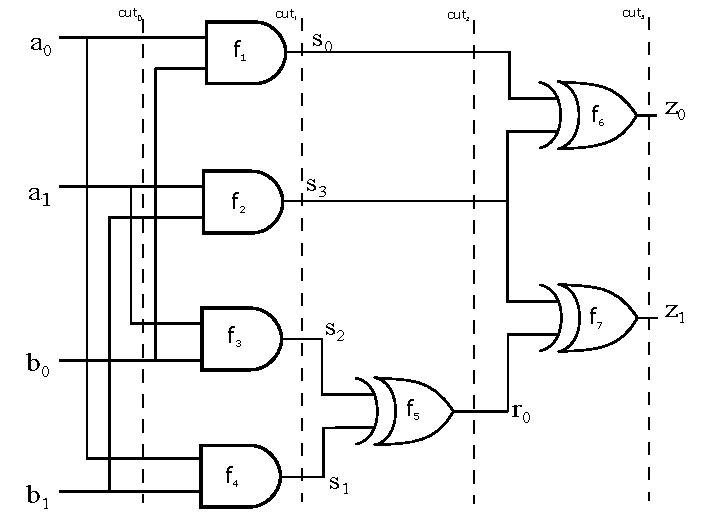
\includegraphics[scale = 0.65]{mas_c}
	\end{center}
	\vspace{-2ex}
	\caption{2-bit Mastrovito multiplier}
	\label{mas_c}
	\vspace{-1ex}
\end{figure}\\
% For the given circuit, we define \textit{cuts} across the gates based on heuristics such as dependency and levelization\cite{maciej:2016:1}. A $cut$ is defined as a set of signals that separates primary inputs from primary outputs. The prominence of these cuts is to maintain a variable order across cuts . For example at each cut $cut_m$ from the figure(\ref{tianka_ckt_c}), the following variable set has to be maintained across reductions.
% \begin{equation}
% \begin{split}
% cut_0 = \{a,b,c\} &\quad cut_3= \{z_1,z_2\}\\
% cut_1 = \{e_0,e_1,c,e_2\}  &\quad cut_4 = \{z\} \\
% cut_2 = \{e_0,d_0,e_2\}
% \end{split}
% \end{equation}
The 2x2 Mastrovito multiplier with specification $f: Z + A\cdot B$, is constructed as follows:
% \begin{lalign*}
% \begin{split}
\begin{enumerate}
    \item{Field construction: $\F_4 = \F_2[X]$ (mod $\mathcal{P}$); where $\mathcal{P} = X^2 + X + 1$ is the primitive polynomial used.}
    \item{$Z = z_0 + z_1*\al; A = a_0 + a_1*\al; B = b_0 + b_1*\al;$ are the word level polynomials, and $\al$ is the root of primitive polynomial s.t. $\mathcal{P}(\al)=0$.}
\end{enumerate}
Based on the circuit topology, RTTO$>$ with variable order:
$\{Z\}>\{A>B\}>\{z_0>z_1\}>\{r_0>s_0>s_3\}>\{s_1>s_2$ $\}>\{a_0>a_1>b_0>b_1\}$\\ 
Let $F$ be the set of all polynomials implementing the circuit which are given as:
% \begin{equation*}
% \begin{split}
% f_1:s_0 + a_0*b_0;  &  f_5:r_0 + s_1 + s_2; & f_8:A + a_0 + a_1*\al; \\
% f_2:s_3 + \mathcal{F}(a_1,b_1);  &  f_6:z_0 + s_0 + s_3; & f_9:B + b_0 + b_1*\al;\\
% f_3:s_2 + a_1*b_0;  &  f_7:z_1 + r_0 + s_3; & f_{10}:Z + z_0 + z_1*\al;\\
% f_4:s_1 + a_0*b_1;
% \end{split}
% \begin{equation}
{\small\begin{flalign*}
f_1:s_0 + a_0*b_0;  &\quad  f_5:r_0 + s_1 + s_2; & f_8:A + a_0 + a_1*\al;\\
% f_2:s_3 + \mathcal{F}(a_1,b_1);  &\quad  f_6:z_0 + s_0 + s_3; & f_9:B + b_0 + b_1*\al;\\
f_2:s_3 + P;  &\quad  f_6:z_0 + s_0 + s_3; & f_9:B + b_0 + b_1*\al;\\
f_3:s_2 + a_1*b_0;  &\quad  f_7:z_1 + r_0 + s_3; & f_{10}:Z + z_0 + z_1*\al;\\
f_4:s_1 + a_0*b_1;
\end{flalign*}}%
We shall add the ideal of vanishing polynomials $J_0$ for primary inputs, outputs, and intermediate variables.  
{\small\begin{flalign*}
f_{11}:a_0^2 + a_0; &\quad f_{15}:s_0^2 + s_0;\quad f_{19}:r_0^2 + r_0;\quad f_{23}:A^4 + A;\\
f_{12}:a_1^2 + a_1; &\quad f_{16}:s_1^2 + s_1;\quad f_{20}:z_0^2 + z_0;\quad f_{24}:B^4 + B;\\
f_{13}:b_0^2 + b_0; &\quad f_{17}:s_2^2 + s_2;\quad f_{21}:z_1^2 + z_1;\\
f_{14}:b_1^2 + b_1; &\quad f_{18}:s_3^2 + s_3;\quad f_{22}:Z^4 + Z;
\end{flalign*}}%
\begin{small}
$F = \{f_1,\dots,f_{10}\}; J = \langle F\rangle = \langle f_1,\dots,f_{10}\rangle; J_0 = \langle f_{11},\dots,f_{24}\rangle$
\end{small}
% Due to RTTO$>$, the set of polynomials ($J+J_0$) is in itself a \Grobner basis.\\

For a correct implementation, specification $f$ vanishes on circuit implementation:
% \begin{equation}
$f \in \langle f_1,f_2,f_3,\dots,f_{10}\rangle+\langle f_{11},f_{12}$ $,\dots,f_{24}\rangle$,
% \end{equation}
 where tail of $f_2$ is unknown.
% h_4f_4 \in \langle f,f_1,f_2,f_3,f_5,f_6,f_7\rangle\\
% h_4f_4 = f+h_1f_1+h_2f_2+h_3f_3+h_5f_5+h_6f_6+h_7f_7

We know that under RTTO$>$, the given set of circuit polynomials in itself form a $GB$. Hence to compute $g$, we start reducing the specification polynomial $f$ using polynomials from the set $\langle J + J_0\rangle$. We will use the following notations for reduction: '[]' to represent quotient-$h_i$'s, '()' to represent divisor-$f_i$'s, and '\{\}' to represent the partial remainder of every reduction step-$fp_i$'s.

\begin{small}
% \begin{split}
$f\xrightarrow[]{f_{10}}[1](Z + z_0 + z_1*\al)+\{ A*B+z_0+\al*z_1\}\rightarrow fp_1$

$fp_1\xrightarrow[]{f_8}[B](A+a_0+\al*a_1)+\{B*a_0+\al*B*a_1+z_0+\al*z_1\}\rightarrow fp_2$

$fp_2\xrightarrow[]{f_9}[a_0+\al*a_1](B+b_0+\al*b_1)+\{z_0+\al*z_1+a_0*b_0+\al*a_0*b_1+\al*a_1*b_0+(\al+1)*a_1*b_1\}\rightarrow fp_3$

$fp_3\xrightarrow[]{f_6}[z_0+s_0+s_3](1)+\{\al*z_1+s_0+s_3+a_0*b_0+\al*a_0*b_1+\al*a_1*b_0+(\al+1)*a_1*b_1\}\rightarrow fp_4$

$fp_4\xrightarrow[]{f_7}[z_1+r_0+s_3](\al)+\{\al*r_0+s_0+(\al+1)*s_3+a_0*b_0+\al*a_0*b_1+\al*a_1*b_0+(\al+1)*a_1*b_1\}\rightarrow fp_5$

$fp_5\xrightarrow[]{f_5}[r_0+s_1+s_2](\al)+\{s_0+(\al+1)*s_3+\al*s_1+\al*s_2+a_0*b_0+\al*a_0*b_1+\al*a_1*b_0+(\al+1)*a_1*b_1\}\rightarrow fp_6$

$fp_6\xrightarrow[]{f_1}[s_0+a_0*b_0](1)+\{(\al+1)*s_3+\al*s_1+\al*s_2+\al*a_0*b_1+\al*a_1*b_0+(\al+1)*a_1*b_1\}\rightarrow fp_7$

% $fp_6\quad\xrightarrow[]{lt(f_2)}[s_3](\underbrace{x+1}_\text{$h_2$})+\{\underbrace{(x)*s_1+(x)*s_2+(x)*a_0*b_1+(x)*a_1*b_0+(x+1)*a_1*b_1}_\text{$g$}\}$
${\scriptstyle fp_7}\xrightarrow[]{{\scriptstyle lt(f_2)}}[{\scriptstyle s_3}](\underbrace{{\scriptstyle \al+1}}_\text{$h_2$})+\{\underbrace{{\scriptstyle\al s_1+\al s_2+\al a_0b_1+\al a_1b_0+(\al+1)a_1b_1}}_\text{$g$}\}$


% \end{split}
\end{small}
Reduction order for $f:$
$f\xrightarrow[]{f_{10}}\xrightarrow[]{f_8}\xrightarrow[]{f_9}\xrightarrow[]{f_6}\xrightarrow[]{f_7}\xrightarrow[]{f_5}\xrightarrow[]{f_1}\xrightarrow[]{lt(f_2)}g$

% \begin{equation}
% \begin{split}
% h_4f_4+h_1f_1+h_2f_2+h_3f_3 = f+h_5f_5+h_6f_6+h_7f_7;\\
% h_4(d_0+P(e_1,c))+h_1f_1+h_2f_2+h_3f_3 = f+h_5f_5+h_6f_6+h_7f_7;\\
% h_4*d_0+h_4*P(e_1,c)+h_1f_1+h_2f_2+h_3f_3 = f+h_5f_5+h_6f_6+h_7f_7;\\
% h_4*P(e_1,c)+h_1f_1+h_2f_2+h_3f_3 = h_4*d_0+f+h_5f_5+h_6f_6+h_7f_7;\\
% h_4*P(e_1,c)+h_1f_1+h_2f_2+h_3f_3 = e_0*e_2+a*c+a+b*c+b+c;\\
% h_4*P(e_1,c)+h_1f_1+h_2f_2+h_3f_3 = e_0*e_2+a*c+a+b*c+b+c;
% \end{split}
% \end{equation}
Since, we know $g,h_2,f_3,f_4,J_0$, we can formulate it as ideal membership testing problem using~\eqref{member}:
\begin{center}
$g \in \langle h_2,f_3,f_4\rangle + \langle J_0\rangle$
\end{center}

This ideal membership test can be done using $lift$ procedure in SINGULAR~\cite{DGPS_410}. The procedure takes polynomial $f$, and ideal $J$ in row matrix form($[J+J_0]$) as inputs, and returns a column matrix $[U]$ as output such that:
\begin{small}
$f = [U]\cdot [J+J_0]$
\end{small}

% \begin{equation}
% \begin{split}
\begin{small}
$g = \begin{bmatrix} h_2^{'} & h_3^{'} & \dots & H \end{bmatrix} \cdot 
    \begin{bmatrix} h_2 \\ f_3 \\ \vdots \\ x_n^2 + x_n \end{bmatrix}$
\end{small}

The matrix output can be written in a linear combination as follows: 
% \end{split}
% \end{equation}
\begin{small}
$\al*s_1+\al*s_2+\al*a_0*b_1+\al*a_1*b_0+(\al+1)*a_1*b_1 = [\al*s_1+\al*s_2+\al*a_0*b_1+\al*a_1*b_0+(\al+1)*a_1*b_1](\al+1) + [0](s_2 + a_1*b_0) + [0](s_1 + a_0*b_1) + \dots + [0](x_n^2 + x_n)$;
\end{small}

The $lift$ procedure uses $GB$ to compute the linear combination. Since the generator set has a constant polynomial($\al+1$), the procedure considers it as constant one during membership computation. Hence the output in this case will be a 1x1 matrix with $g$ itself projected as the solution. To normalize the ignored constant, we need to divide(multiply the inverse) the solution $g$ by the constant$(\al+1)$ and reduce it with polynomials \{$f_3,f_4$\} in order to arrive at a implementable solution.

\begin{small}
$(\al+1)^{-1} = \al$

$h_2^{''} = \al*h_2^{'} = \al*(\al*s_1+\al*s_2+\al*a_0*b_1+\al*a_1*b_0+(\al+1)*a_1*b_1)$

$h_2^{''} = (\al+1)*s_1+(\al+1)*s_2+(\al+1)*a_0*b_1+(\al+1)*a_1*b_0+ a_1*b_1$

$h_2^{''}\xrightarrow[]{f_{3}}\xrightarrow[]{f_4}\underbrace{a_1*b_1}_\text{P}$
\end{small}

This computed $P$ is a valid solution and can be used as tail of $f_2$. If the resulting $P$ were not a solution in immediate support variables of $s_3$($a_1,b_1$), we could have arrived at this desired solution by devising a new term order. The new term order will have variables $(s_3,a_1,b_1)$ moved to the end on the variable order. We could then compute a $GB$ using the modified term order with the intermediate solution $P$ added as tail of $f_2$. This $GB$ will have one and only one polynomial which is of the form $s_3 + \mathcal{F}(a_1,b_1)$, where $\mathcal{F}$ is the function implemented by the gate for these variables.\\
Modified term order $\{Z\}>\{A>B\}>\{z_0>z_1\}>\{r_0>s_0\}>\{s_1>s_2$ $\}>\{a_0>b_0>s_3>a_1>b_1\}$.\\
To illustrate the computation of multiple solutions, let's take the current solution $a_1*b_1$ as our $P$. With RTTO$>$ as our term order, from~\eqref{quotcomp}:

$a_1*b_1 - P^{'} \in \{f_3,f_4,x_l^q-x_l\}:h_2$;\\
The result from quotient of ideal operation is given as:
{\small\begin{flalign*}
f_3:s_2 + a_1*b_0;  f_{13}:b_0^2 + b_0; f_{23}:A^4 + A;\\
f_4:s_1 + a_0*b_1;  f_{14}:b_1^2 + b_1; f_{24}:B^4 + B; \\
f_{11}:a_0^2 + a_0; f_{16}:s_1^2 + s_1; \\
f_{12}:a_1^2 + a_1; f_{17}:s_2^2 + s_2;
\end{flalign*}}%
Any polynomial from the above list when added in tail of $f_2$ along with $P$ satisfies the solution set for the given unknown component.
\end{Example}

\subsection{Circuit implementation as reference}
Consider a circuit implementation $C$, modeled as polynomials $F = \{f_1,\dots,f_s\}\in \mathbb{F}_q[in_j,x_1,\dots, x_n]$, with $J_1=\langle F \rangle$, $in_j$ as the set of all primary inputs, and $x_n$ as the word level output. Let us assume $f_i:1\le i \le s$ to be the unknown component which is of the special form:
\begin{gather*} 
f_i = x_k + P
\end{gather*}

Let us consider a different circuit $C_1$ as the golden specification which implements the same function as $C$. The reference circuit is modeled as polynomials $Q = \{q_1,\dots q_r\}\in \mathbb{F}_q[in_j,y_1,\dots, y_m]$, with $J_2=\langle Q \rangle$, $in_j$ as the set of all primary inputs, and $y_m$ as the word level output.

To formulate the problem, we will derive a new circuit structure using the above two implementations ($C,C_1$). Primary input set $in_j$ will be used as the common set of inputs for both the circuits, and the word level outputs ($x_n,y_m$) will be mitered using an XOR gate. A new specification polynomial $f$ is derived using the above setup as:
\begin{gather}
f : t*(x_n-y_m)
\end{gather}

where, $t$ is the final output of miter gate.

Now, for a correct implementation, specification $f$ should vanish on the variety of ideal generated by the circuit polynomials i.e., $f$ will be in the ideal generated by the circuit:

$f \in J_1 + J_2 + J_0$: where $J_0$ is the set of all vanishing polynomials from circuits $C$, $C_1$ and miter output $t$.

{\small $f \in \langle f_1,\dots,f_s\rangle + \langle q_1,\dots,q_r\rangle + \langle x_l^q-x_l\rangle + \langle y_u^q-y_u\rangle + \langle t^q-t\rangle$; $1\le l \le n,1\le u \le m$}

The problem formulation is now exactly same as~\eqref{member} with $f_i$ from circuit $C$ as the unknown gate. Now, we will follow the same procedure as in the first notion to realize the function of the unknown component. Once a solution has been computed, we can verify the circuit using principles from weak $\it{Nullstellensatz}$ by checking if $GB(J_1+J_2+J_0)=\{1\}$.

% \begin{algorithm}
% \caption{Resolve the unknown component for a given circuit}
% \label{algo:unknownComponent}
% \begin{algorithmic}[1]

% \Procedure{$multi\_variate\_division$}{$F,f$}

% \Procedure{$forward\_lifting$}{}

% \EndProcedure
% \end{algorithmic}
% \end{algorithm}

% Thus, $P(u_1)=P(e_1,c)=c$, which can implemented as a simple AND gate with $c$ as both inputs. 

% \begin{figure}[ht]
% 	\begin{center}
% 	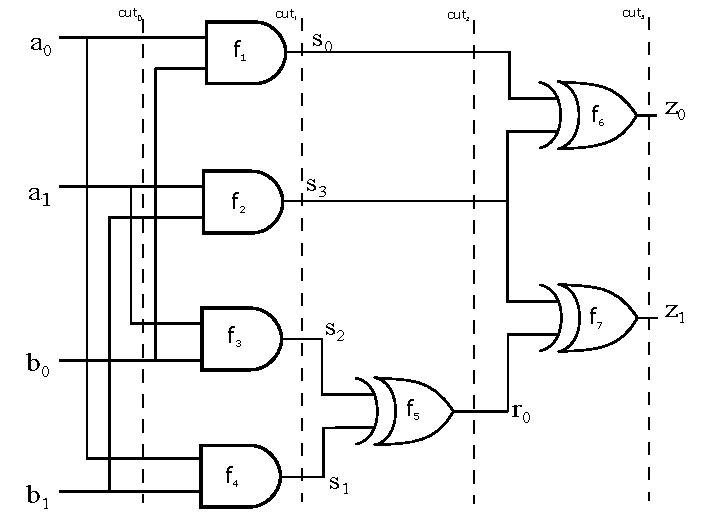
\includegraphics[scale = 0.40]{mas_c}
% 	\end{center}
% 	\vspace{-1ex}
% 	\caption{correct implementation mastrovito}
% 	\label{mas_c}
% 	\vspace{-1ex}
% \end{figure}

% \begin{figure}[ht]
% 	\begin{center}
% 	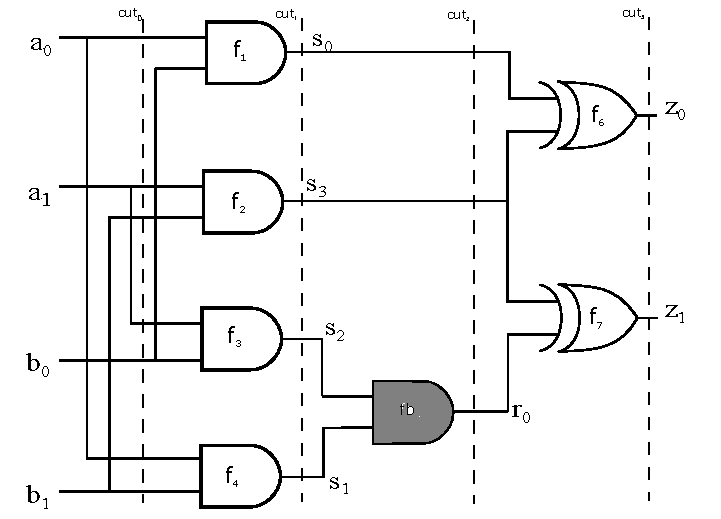
\includegraphics[scale = 0.40]{mas_b}
% 	\end{center}
% 	\vspace{-4ex}
% 	\caption{buggy implementation mastrovito}
% 	\label{mas_b}
% 	\vspace{-2ex}
% \end{figure}
%\section{Experiments}
\label{sec:exp}

This section presents experimental results using our approach to debug
the circuits and perform a single-fix rectification. 
We compare results of our implementation against the incremental SAT-based approach presented in~\cite{fujita:2015} wherever it's relevant.
The approach presented in~\cite{fujita:2015} is implemented using PICOSAT~\cite{picosat}. The experiments were performed on a 3.5GHz 
Intel(R) $\text{Core}^{\text{TM}}$ i7-4770K Quad-Core CPU with 32 GB of RAM. The data-path sizes {$k$} are selected according to cryptography standards recommended by U.S. National Institute of Standards and Technology (NIST). 
% In our experiments, the labels $NO$, $NM$, and $NI$ denote 
% % the location of unknown component within the circuit topology. Here $NI$, $NM$, and $NO$ 
% that the unknown component is near the input, middle, and near the output, respectively.
We have performed experiments for the cases when the bugs  are present near 
the input, middle, or near the output of the circuit, represented
using labels $NI$, $NM$, and $NO$ respectively in the tables. All the algorithms
were implemented in SINGULAR~\cite{DGPS}. 

%\subsection{Word level specification v/s Gate level implementation}

\subsubsection{Verification between a word level specification v/s Mastrovito implementation}
~\autoref{masvsspec} presents the results of our approach when the bugs are placed
in a Mastrovito multiplier implementation compared against a specification, which is given in terms of a word level polynomial $f$. 
A Mastrovito multiplier has word level specification $Z = A\times B \pmod{ P(x)}$, 
where $P(x)$ is a given primitive polynomial for the datapath size $k$. The product $A \times B$ 
is computed using an array multiplier architecture, and then the result is reduced modulo $P(x)$. 
Bugs in the circuit are introduced, and the presence of the bugs is
detetced. Then we apply our approach to check for single-fix
rectification interatively on the nets selected in $\mathcal{N}$. If
rectification is feasible at $x_i$, the unknown component problem is
solved to identify a rectification function. 

%% The circuit implementation is modeled as a set of polynomials $F=\{f_1,\dots f_i,\dots,f_s\}$. The 
%% approach then follows the partial reduction of specification polynomial $f$ until leading term of $f_i$ while
%% recording the intermediate quotients and remainders. We then represent the partial remainder as a linear combination
%% using the remaining gate polynomials and the quotient to obtain the solution $P$.
We 
are able to verify and debug the circuits for upto 64-bits within our
stipulated Time Out ($TO$)  period.

\begin{table*}[hbt]
\centering
\caption{{\small Single fix rectification debug in Mastrovito circuit against word level specification}. Time is in seconds; $k$ = Datapath Size, \#Gates = No. of gates, K = $10^3$, \textit{a}=verification time, \textit{b}=time for rectification check, \textit{c}=time for component correction computation,\textit{d}=total time}
\label{masvsspec}
\begin{tabular}{| c | c | c | c | c | c | c | c | c | c | c | c | c | c |} \hline
\multirow{3}{*}{\textbf{k}}& \multirow{3}{*}{\#Gates} & \multicolumn{12}{ c |}{Our implementation}\\ \cline{3-14}
&&\multicolumn{4}{ c |}{\it NI}&\multicolumn{4}{ c |}{\it NM}&\multicolumn{4}{ c |}{\it NO}\\ \hline
&&{\it a}&{\it b}&{\it c} &{\it d}&{\it a}&{\it b}&{\it c} &{\it d}&{\it a}&{\it b}&{\it c} &{\it d}\\ \hline
9 & 0.23K & 0.0 & 0.0 & 0.0 & 0.0 & 0.0 & 0.0 & 0.0 & 0.0 & 0.0 & 0.0 & 0.0  & 0.0\\ \hline
10& 0.29K & 0.0 & 0.0 & 0.0 & 0.0 & 0.0 & 0.0 & 0.0 & 0.0 & 0.0 & 0.0 & 0.0  & 0.0\\ \hline
11& 0.35K & 0.0 & 0.0 & 0.1 & 0.1 & 0.0 & 0.0 & 0.1 & 0.1 & 0.0 & 0.0 & 0.1  & 0.1\\ \hline
12& 0.97K & 0.1 & 0.5 & 0.4 & 0.9 & 0.2 & 0.5 & 0.4 & 1.1 & 0.5 & 0.8 & 0.4  & 1.7\\ \hline
13& 0.82K & 0.1 & 0.3 & 0.2 & 0.6 & 0.2 & 0.6 & 0.2 & 1.0 & 0.7 & 0.8 & 0.2  & 1.7\\ \hline
16& 1.8K  & 0.9 & 2.6 & 1.0 & 4.5 & 1.1 & 3.5 & 1.0 & 5.6 & 2.8 & 5.3 & 1.0  & 9.1\\ \hline
32& 5.4K  & 36  & 110 & 42  & 188 & 40  & 160 & 47  & 247 & 38  & 240 & 150  & 428\\ \hline
64& 21.8K & 2210& 7100 & 2432 & 9532 & 2200 & 8000 & 2575 & 12775 & 2150& 7840 & 10020 & 20010 \\ \hline
\end{tabular}
\end{table*}


\begin{table*}[hbt]
\centering
\caption{{\small Rectification for Mastrovito circuit with Montgomery circuit as specification}. Time is in seconds; $k$ = Datapath Size, \#Gates = No. of gates, (TO): Time-Out = 3 hrs, K = $10^3$,\textit{a}=verification time, \textit{b}=time for rectification check, \textit{c}=time for component correction computation, \textit{d}=total time}
\label{masusmontspec}
\begin{tabular}{| c | c |  c | c | c | c | c | c | c | c | c | c | c | c | c | c | c |} \hline
\multirow{4}{*}{\textbf{k}}& \multirow{4}{*}{\#Gates} & \multicolumn{3}{ c |}{Incremental SAT\textbf{~\cite{fujita:2015}}}& \multicolumn{12}{ c |}{Our Approach}\\ \cline{3-17}
&&\multirow{2}{*}{\it NI}&\multirow{2}{*}{\it NM}&\multirow{2}{*}{\it NO}&\multicolumn{4}{ c |}{\it NI}&\multicolumn{4}{ c |}{\it NM}&\multicolumn{4}{ c |}{\it NO} \\ \cline{6-17}
&&&&&{\it a}&{\it b}&{\it c} &{\it d}&{\it a}&{\it b}&{\it c} &{\it d}&{\it a}&{\it b}&{\it c} &{\it d}\\ \hline
9 & 0.6K & 35   & 37   & 33    & 0.1 & 0.5 & 0.2 & 0.8 & 0.2 & 0.2 & 0.1 & 0.5 & 1.8 & 2.2 & 0.6 & 4.6 \\ \hline
10& 0.7K & 231  & 215  & 214   & 0.3 & 1   & 0.5 & 1.8 & 0.3 & 1   & 0.8 & 2.1 & 4.7 & 5.4 & 0.2 & 10 \\ \hline
11& 0.9K & 2090 & 1927 & 2000  & 0.6 & 2   & 1   & 3.6 & 0.8 & 2   & 32  & 35  & 9 & 10 & 0.4 & 19 \\ \hline
12& 1.6K & 8676 & 23400& 24085 & 3.2 & 9.6 & 3.5 & 16  & 3.2 & 9.3 & 12  & 24  & 155 & 160 & 1.6 & 316 \\ \hline
13& 1.7K & TO   & TO   & TO    & 3.3 & 10  & 4.5 & 18  & 3.5 & 10 & 22 & 35 & 170 & 177 & 1.6 & 349 \\ \hline
16& 3K   & TO   & TO   & TO    & 27  & 81  & 35  & 143 & 28 & 83 & 48 & 159 & 210 & 176 & 2.5 & 389\\ \hline
32& 9.8K & TO   & TO   & TO    &  2060   & 6595    & 1870&  10525   & 2100 & 7320 & 1289 & 10709 & 2215 & 7870 & 1204 & 11289 \\ \hline
\end{tabular}
\end{table*}




% \begin{table}[H]
% \centering
% \caption{{Single fix rectification debug in Mastrovito circuit against word level specification}. Time is in seconds; $k$ = Datapath Size, \#Gates = No. of gates, K = $10^3$}
% \label{masvsspec}
% \begin{tabular}{| c | c | c | c | c | c | c | c | c | c | c | c | c | c | c | c | c |} \hline
% \multirow{3}{*}{\textbf{k}}& \#Gates & \multicolumn{15}{ c |}{Our implementation}\\ \cline{3-17}
% &&\multicolumn{5}{ c |}{\it NI}&\multicolumn{5}{ c |}{\it NM}&\multicolumn{5}{ c |}{\it NO}\\ \hline
% &&{\it a}&{\it b}&{\it c} &{\it d}&{\it e}&{\it a}&{\it b}&{\it c} &{\it d}&{\it e}&{\it a}&{\it b}&{\it c} &{\it d}&{\it e}\\ \hline
% 9& 0.23K & 0.0 & 0.1 & 0.0 & 0.2 & 0.0 & 0.1 & 0.0 & 0.2 & 0.0 & 0.2 & 0.0 & 0.3\\ \hline
% 10& 0.29K & 0.0 & 0.3 & 0.0 & 0.3 & 0.0 & 0.3 & 0.0 & 0.3 & 0.0 & 0.4 & 0.0 & 1.4\\ \hline
% 11& 0.35K & 0.0 & 0.2 & 0.0 & 0.3 & 0.0 & 0.3 & 0.0 & 0.4 & 0.0 & 0.6 & 0.0 & 0.7\\ \hline
% 12& 0.97K & 0.1 & 7.5 & 0.5 & 8.0 & 0.2 & 10.1 & 0.5 & 10.5 & 0.5 & 121.2 & 0.8 & 121.3\\ \hline
% 13& 0.82K & 0.1 & 4.3 & 0.3 & 4.5 & 0.2 & 11.3 & 0.6 & 11.2 & 0.7 & 156.3 & 0.8 & 158.1\\ \hline
% 16& 1.8K & 0.9 & 14.1 & 2.6 & 30.2 & 1.1 & 33.1 & 3.5 & 34.9 & 2.8 & 501.2 & 5.3 & 503.0\\ \hline
% 32& 5.4K & 36.8 & 378.6 & 110.5 & 544.7 & 40.0 & 567.1 & 160.3 & 767.2 & 38.1 & 1286.1 & 240.3 & 1342.7\\ \hline
% %64& 21.8K & 36.8 & 378.6 & 110.5 & 544.7 & 40.0 & 567.1 & 160.3 & 767.2 & 38.1 & 1286.1 & 240.3 & 1342.7\\ \hline
% \end{tabular}
% \end{table}

\subsubsection{Word level specification v/s Point addition implementation}
Point addition is an important operation required for the task of encryption, decryption 
and authentication in Elliptic Curve Cryptography (ECC). 
Modern approaches represent the points in projective
coordinate systems, {\it e.g.}, the L$\acute{o}$pez-Dahab (LD) projective coordinate, due to which the point addition 
operation can be implemented as polynomials in the field.

\begin{Example}
{\it\small %Consider point addition in L$\acute{o}$pez-Dahab (LD) projective
  %coordinate.
  Given an elliptic curve: $Y^2 + XYZ = X^3Z + aX^2Z^2 +
  bZ^4$ over $\mathbb{F}_{2^k}$, where $X,Y,Z \in \mathbb{F}_{2^k}$ and similarly, $a, b$ are
  constants from the field. Point addition over the
  elliptic curve is ($X_3$, $Y_3$, $Z_3$) = ($X_1$, $Y_1$, $Z_1$) +
  ($X_2$, $Y_2$, $1$).  Then $X_3$, $Y_3$, $Z_3$ can be computed as
  follows:}
\vspace{-0.09in}
{\tiny
\begin{align*}
&A = Y_2 \cdot Z_1^2 + Y_1  &&B = X_2 \cdot Z_1 + X_1 \\
&C = Z_1 \cdot B  &&D = B^2 \cdot(C + a Z_1^2) \\
&Z_3 = C^2 && E = A \cdot C  \\
&X_3 = A^2 + D + E &&F = X_3 + X_2 \cdot Z_3 \\
&G = X_3 + Y_2\cdot Z_3 && Y_3 = E\cdot F + Z_3 \cdot G
\end{align*}
}
\vspace{-0.38in}

\end{Example}

Each of the polynomials in the above design are implemented as a
(gate-level) logic block and are interconnected to obtain final
outputs $X_3,Y_3$ and $Z_3$. ~\autoref{pdvsspec} shows
the comparison of the time required for debugging and rectification
for the implementation of the block $D= B^2\cdot(C + aZ_1^2)$. 

\begin{table}[H]
\centering
\caption{{\small Single fix rectification debug in Point Addition circuits against word level specification}. Time is in seconds; $k$ = Datapath Size, \#Gates = No. of gates, K = $10^3$, \textit{a}=verification time, \textit{b}=time for rectification check,\textit{c}=time for component correction computation,\textit{d}=total time}
\label{pdvsspec}
\begin{tabular}{| c | c | c | c | c | c | c | c | c | c | c | c | c | c |} \hline
\multirow{3}{*}{\textbf{k}}& \multirow{3}{*}{\#Gates} & \multicolumn{12}{ c |}{Our implementation}\\ \cline{3-14}
&&\multicolumn{4}{ c |}{\it NI}&\multicolumn{4}{ c |}{\it NM}&\multicolumn{4}{ c |}{\it NO}\\ \hline
&&{\it a}&{\it b}&{\it c} &{\it d}&{\it a}&{\it b}&{\it c} &{\it d}&{\it a}&{\it b}&{\it c} &{\it d}\\ \hline
8 & 244  & 0.0 & 0.0 & 0.0 & 0.0 & 0.0 & 0.0 & 0.0 & 0.0 & 0.0 & 0.0 & 0.0 & 0.0\\ \hline
16& 1.2K & 1.3 & 3.9 & 1.5 & 6.7 & 1.2 & 3.7 & 2   & 6.9 & 1.2 & 3.7 & 1.8 & 6.7\\ \hline
32& 3.9K & 37  & 112 & 77  & 226 & 38  & 110 & 22  & 170 & 37  & 108 & 35  & 180\\ \hline
%64& 15K  & 40  & 2283&  &  &  &  &  &  &  &  &   & \\ \hline
\end{tabular}
\end{table}

\subsubsection{Word level specification v/s Barrett reduction implementation}
Barrett reduction
%~\cite{barrett}
is the other widely used multiplier design
method adopted in cryptography system designs. 
Based on Barrett reduction, a multiplier can be designed in two steps:
multiplication $R = A \times B$ and a subsequent Barrett reduction G =
R (mod P). ~\autoref{bartvsspec} shows results for debugging and rectification of
Barrett multipliers against a polynomial specification. 

\begin{table}[H]
\centering
\caption{{\small Single fix rectification debug in Barrett reduction circuits against word level specification}. Time is in seconds; $k$ = Datapath Size, \#Gates = No. of gates, K = $10^3$, \textit{a}=verification time, \textit{b}=time for rectification check,\textit{c}=time for component correction computation,\textit{d}=total time}
\label{bartvsspec}
\begin{tabular}{| c | c | c | c | c | c | c | c | c | c | c | c | c | c |} \hline
\multirow{3}{*}{\textbf{k}}& \multirow{3}{*}{\#Gates} & \multicolumn{12}{ c |}{Our implementation}\\ \cline{3-14}
&&\multicolumn{4}{ c |}{\it NI}&\multicolumn{4}{ c |}{\it NM}&\multicolumn{4}{ c |}{\it NO}\\ \hline
&&{\it a}&{\it b}&{\it c} &{\it d}&{\it a}&{\it b}&{\it c} &{\it d}&{\it a}&{\it b}&{\it c} &{\it d}\\ \hline
8 & 134 & 0.0 & 0.0 & 0.0 & 0.0 & 0.0 & 0.0 & 0.0 & 0.0 & 0.0 & 0.0 & 0.0 & 0.0\\ \hline
16& 427 & 0.1 & 0.0 & 0.0 & 0.1 & 0.0 & 0.2 & 0.1 & 0.3 & 0.0 & 0.1 & 0.3 & 0.4\\ \hline
32& 1.4K & 0.4 & 1.4 & 0.1 & 1.9 & 0.5 & 1.5 & 0.1 & 2.1 & 1.2 & 2.2 & 1.1 & 4.5\\ \hline
64& 4.9K & 19  & 58  & 5.4 & 82  & 21  & 60  & 1.7 & 83  & 63  & 104 & 141 & 308\\ \hline
\end{tabular}
\end{table}

Since the SAT-based approach cannot be applied against a word level specification polynomial, 
we perform experiments while using another multiplier implementation as the specification.

\subsubsection{Verification between a specification and implementation
  given as gate level circuits: Mastrovito v/s Montgomery multipliers}

%% \begin{table*}[ht]
%% \centering
%% \caption{{Resolving Unknown Component in Mastrovito circuit with Montgomery circuit as specification}. Time is in seconds; $k$ = Datapath Size, \#Gates = No. of gates, (TO): Time-Out = 3 hrs, K = $10^3$,\textit{a}=verification time, \textit{b}=time for rectification check,\textit{c}=time for component correction computation,\textit{d}=total time}
%% \label{masusmontspec}
%% \begin{tabular}{| c | c |  c | c | c | c | c | c | c | c | c | c | c | c | c | c | c |} \hline
%% \multirow{4}{*}{\textbf{k}}& \multirow{4}{*}{\#Gates} & \multicolumn{3}{ c |}{Incremental SAT\textbf{~\cite{fujita:2015}}}& \multicolumn{12}{ c |}{Our Approach}\\ \cline{3-17}
%% &&\multirow{2}{*}{\it NI}&\multirow{2}{*}{\it NM}&\multirow{2}{*}{\it NO}&\multicolumn{4}{ c |}{\it NI}&\multicolumn{4}{ c |}{\it NM}&\multicolumn{4}{ c |}{\it NO} \\ \cline{6-17}
%% &&&&&{\it a}&{\it b}&{\it c} &{\it d}&{\it a}&{\it b}&{\it c} &{\it d}&{\it a}&{\it b}&{\it c} &{\it d}\\ \hline
%% 9 & 0.6K & 35   & 37   & 33    & 0.1 & 0.5 & 0.2 & 0.8 & 0.2 & 0.2 & 0.1 & 0.5 & 1.8 & 2.2 & 0.6 & 4.6 \\ \hline
%% 10& 0.7K & 231  & 215  & 214   & 0.3 & 1   & 0.5 & 1.8 & 0.3 & 1   & 0.8 & 2.1 & 4.7 & 5.4 & 0.2 & 10 \\ \hline
%% 11& 0.9K & 2090 & 1927 & 2000  & 0.6 & 2   & 1   & 3.6 & 0.8 & 2   & 32  & 35  & 9 & 10 & 0.4 & 19 \\ \hline
%% 12& 1.6K & 8676 & 23400& 24085 & 3.2 & 9.6 & 3.5 & 16  & 3.2 & 9.3 & 12  & 24  & 155 & 160 & 1.6 & 316 \\ \hline
%% 13& 1.7K & TO   & TO   & TO    & 3.3 & 10  & 4.5 & 18  & 3.5 & 10 & 22 & 35 & 170 & 177 & 1.6 & 349 \\ \hline
%% 16& 3K   & TO   & TO   & TO    & 27  & 81  & 35  & 143 & 28 & 83 & 48 & 159 & 210 & 176 & 2.5 & 389\\ \hline
%% 32& 9.8K & TO   & TO   & TO    &     &     & 1870&     &  &  & 1289 &  &  &  & 1204 &  \\ \hline
%% \end{tabular}
%% \end{table*}

%\subsubsection{Mastrovito v/s Montgomery}
%% \begin{figure}[H]
%%   \centering
%%   %\def\svgwidth{340pt}
%%   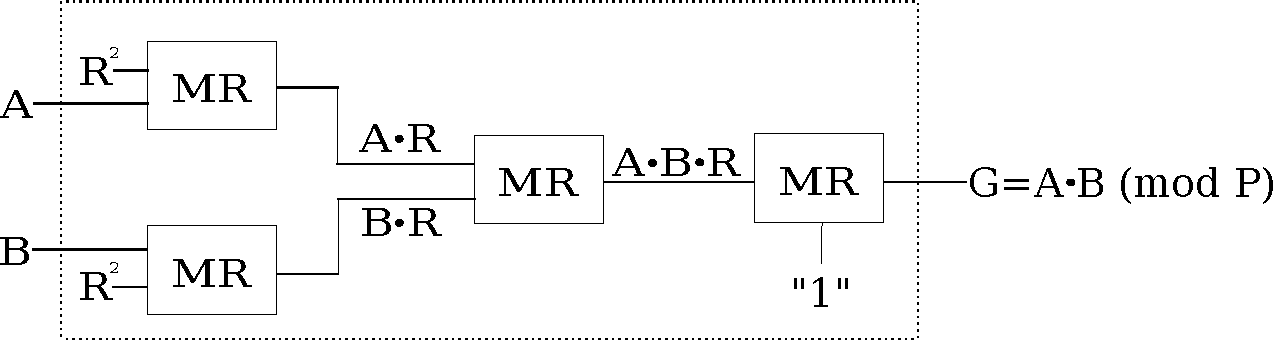
\includegraphics[scale=0.34]{new_mmcircuit-eps-converted-to}
%%   \caption{Montgomery multiplication.}
%%   \label{montfig}
%%   \end{figure}

Montgomery architectures~\cite{acar:1998},~\cite{wu:2002},
% \cite{Barrett:1987} 
~\cite{knezevic:2008} are considered more efficient than Mastrovito multipliers for exponentiation, 
as they do not require explicit reduction modulo $P(x)$ after each step.
%% ~\autoref{montfig} shows the structure of a Montgomery
%% multiplier. Each MR block computes $A\cdot B\cdot R^{-1}$, where $R$
%% is selected as a power of a base ($\alpha^{k}$) and $R^{-1}$ is the multiplicative 
%% inverse of $R$ in $\mathbb{F}_{2^k}$. As this operation cannot compute $A\cdot B$
%% directly, we need to pre-compute $A\cdot R$ and $B\cdot R$ as shown in the~\autoref{montfig}. 
%% We denote the leftmost
%% two blocks as Block A (upper) and B (lower), the middle block as Block
%% C and the output block as Block D.
% We have presented results for GBR
%on both \textit{flattened} and \textit{hierarchical} netlists of these
% multipliers.

~\autoref{masusmontspec} presents the results of our approach to debug
and rectification with the bugs placed in the Montgomery multiplier
with a Mastrovito multiplier circuit used as the specification. While
the approach~\cite{fujita:2015} finds a satisfying transformation
assignment which can be mapped to a library gate, our approach debugs
the circuit and finds a single fix rectification function. As shown in
the table, our approach shows improvement by several orders of
magnitude over \cite{fujita:2015}. 

%The comparison of bug placement reflects the complexity involved in
%debugging circuits where the bug lies in the deeper part ($NO$) of the
%topology.
It takes considerable amount of time for verification and
rectification check when the bug is close to the output. We are
working on further improving the experiments by employing better data
structures like  
ZBDDs~(\cite{minato:zbdd}), and devising better heuristics to perform
rectification check.
%We are also looking into efficient
%implementations for representing the partial remainder as a linear
%combination of an ideal during correction computation.
Due to several limitations w.r.t number of ring variables that can be
declared in SINGULAR, we have had to restrict our experiments within
64-bit data-path size.   

\section{Conclusions}

This paper has presented a fully automated debug approach for single fix rectification under RTTO$>$ based on \Grobner basis reductions and ideal
membership test. We presented a procedure to test for the existence of utilized the duality of varieties and ideals to check for the existence of single fix rectification at a given net. 
The experimental results demonstrate the efficacy of our approach for finite field arithmetic circuits where we achieve several orders of magnitude
improvement as compared to recent SAT-based approach. 
As part of our future work, we are working on improving the efficiency of our implementation to target higher bit-widths. We are also investigating how the current procedure can be extended to cover integer arithmetic circuits.
Further research also includes exploring the current approach for
the case of multi-fix rectification.  

%\section{Conclusion and future work}
This paper has presented an approach based on \Grobner basis reductions and ideal
membership test to compute a function implemented by an unknown component in a circuit which models
a given specification. 
% We presented a procedure to systematically use \Grobner basis based reduction and ideal membership testing to arrive at a 
% solution, such that the resulting logic function of the circuit conforms to the reference specification. 
The paper also utilizes the concept of quotient of ideals to derive multiple solutions
for the unknown component. The experimental results demonstrate the efficiency of our approach 
for finite field arithmetic circuits where we achieve several orders of 
magnitude improvement as compared to recent SAT-based approach. 
We also present the theory for exploring the solution for the unknown 
component in terms of its immediate inputs.  
% The most desired solution which is in terms of immediate support 
% variables of the unknown component relies on expensive \Grobner basis re-computation 
% with a different term order. 
% As part of our future work, we are exploring heuristics 
% in order to arrive at a guided, simple implementable solutions set for $P$.
% The current set-up deals with one unknown 
% component or sub-circuit, 
As part of our future work, we are working on extending the current approach  
for the case of multiple independent/dependent bugs in the design along
with identifying the potential locations where the circuit can be rectified 
with the current setup.  
% Also, identifying the bug location, 
% which is the primary concern in the overall scope of automated debugging 
% needs to be addressed as well. 
%%%%%%%%%%%%%%%%%%%% The bibliography %%%%%%%%%%%%%%%%%%%%%%%%%%%%

\bibliographystyle{IEEEtran}
\bibliography{vikas}

\end{document}

%%%%%%%%%%%%%%%%%%%%%%%%%%%  End of IEEEsample.tex  %%%%%%%%%%%%%%%%%%%%%%%%%%%
